\documentclass{beamer}
 
\usepackage[utf8]{inputenc}
\usepackage{hyperref}
\usepackage{listings}
\usepackage{graphicx}

\usetheme{focus}
 
%Information to be included in the title page:
\title{CLTK}
\author{Eleftheria, Clément}
\institute{CLTK}
\date{06/10/2019}


%\lstset{language=TeX}

%\AtBeginSection[]
%{
%\begin{frame}{Plan}
%\tableofcontents[currentsection]
%\end{frame}
%}

\AtBeginSubsection[]
{
\begin{frame}{Plan}
\tableofcontents[currentsubsection]
\end{frame}
}


\newcommand*\rot{\rotatebox{90}}

\hypersetup{
    colorlinks=true,
    linkcolor=blue,  
    urlcolor=cyan,
}

\begin{document}

\begin{frame}
%\titlepage
\begin{center}
    {\large Introduction to CLTK (Classical Language ToolKit)}\\
    Eleftheria Chatziargyriou \& Clément Besnier \\
    06/11/2019 \\
    
\includegraphics[scale=0.5]{cltklogo.png}
\end{center}

\end{frame}

\begin{frame}
\frametitle{Outline}
\tableofcontents
\end{frame}

\section{CLTK: philosophy and organization}

% \begin{frame}
% \frametitle{Brief overview on CLTK}
% %like page 5
% \begin{itemize}
%     \item definition
%     \item license
%     \item started in 2012
%     \item covered languages
%     \item number of citations
% \end{itemize}
% \end{frame}
\subsection{Overview}

\begin{frame}{CLTK}
\begin{itemize}
    \item \textbf{Free and Open-Source} \textbf{Python} library
    %\pause
    \item Founded in 2014 by \textbf{Kyle P. Johnson}
    %\pause
    \item Provides \textbf{NLP\footnote{NLP: Natural Language Processing} tools} for \textbf{historical languages}
    %\pause
    \item \textbf{Shares} a \textbf{high-quality code} for \textbf{academic research}
    
\end{itemize}
%\pause
Co-maintainers: Patrick J. Burns and Kyle P. Johnson.
    
\end{frame}


\begin{frame}
\frametitle{CLTK}
Main goals:
\begin{itemize}
% add examples of analysis-friendly corpora
\item[1.] Compile analysis-friendly corpora
% Examples: 
\item[2.] Collect and generate linguistic data\footnote{\href{https://github.com/cltk/latin_models_cltk}{https://github.com/cltk/latin\_models\_cltk}}
% Example of papers
\item[3.] Act as a free and open platform for generating scientific research

\end{itemize}
    
\end{frame}

\subsection{NLP Tools}
\begin{frame}
\frametitle{CLTK among other NLP Tools in Python}
\begin{itemize}
    
    \item NLP: SpaCy\footnote{\href{https://spacy.io/}{https://spacy.io/}}, NLTK\footnote{\href{https://www.nltk.org/}{https://www.nltk.org/}}, StanfordNLP\footnote{\href{https://stanfordnlp.github.io/stanfordnlp/}{https://stanfordnlp.github.io/stanfordnlp/}}
    %\item Academic research teams focus on one or related languages and do not often share tools to the community  
    \item Python is a programming language widely used by researchers
\end{itemize}
\end{frame}


\subsection{Historical Languages}

\begin{frame}
\frametitle{Historical Languages}
\begin{itemize}
    \item Early Antiquity: Sumerian, Akkadian, Old Egyptian, etc
    \item Late Antiquity: Ancient Greek, Latin, Sanskrit, Classical Chinese, Gothic, etc
    \item Middle Ages: Medieval Latin, Coranic Arabic, Koine, Old and Middle High German, Old Norse, etc
\end{itemize}
\end{frame}

\begin{frame}
\frametitle{Historical Languages}
\begin{itemize}
    \item Handles languages written and spoken before Gutenberg
    \item Documents written in these languages have specific features:   
    \begin{itemize}
        \item often relatively small and fragmentary surviving texts
        \item spelling not normalized
        %\item dialect boundaries not clearly observable
        %\item language evolutions must be taken into account
        \item diachronic component of languages must be handled
        \item no more living speakers
        \item no more produced texts
    \end{itemize}
    \item Expert skills needed
\end{itemize}
\end{frame}


\subsection{High Quality Code}

\begin{frame}
\frametitle{Principles}
\begin{itemize}
    \item Decentralization
    \item Disintermediation
    \item Extensibility
    \item Standardization
    \item Simplicity
\end{itemize}{}
    
\end{frame}


\begin{frame}
\frametitle{Community Design Principles}
\begin{itemize}
    %\item Free \& Open Source
    \item Transparency
    \item Inclusion
    \item Multi-disciplinary
    \item Mutual benefit
\end{itemize}
\end{frame}


\begin{frame}
\frametitle{Free, open-source}
\begin{itemize}
    \item Free  %
    \item MIT license\footnote{\href{https://choosealicense.com/licenses/mit/}{https://choosealicense.com/licenses/mit/}}, you can share and reuse it, even for commercial code
    \item Inclusion % researchers, like students and passionate people
    \item Multi-disciplinary % computer science, linguistics, statistics, history
    %\item Mutual benefit % consequence of the previous remark
\end{itemize}
\end{frame}



\begin{frame}[fragile]
\frametitle{Academic research}

    How to cite the project:
    \begin{lstlisting}[basicstyle=\scriptsize,frame=single]
    @Misc{johnson2014,
        author = {Kyle P. Johnson et al.},
        title = {CLTK: The Classical Language Toolkit},
        howpublished = {\url{https://github.com/cltk/cltk}},
        note = {{DOI} 10.5281/zenodo.<current_release_id>},
        year = {2014--2019},
    }
    \end{lstlisting}
    You can also cite the precise contributors\footnote{\href{https://github.com/cltk/cltk/blob/master/contributors.md}{https://github.com/cltk/cltk/blob/master/contributors.md}} if you use a specific module.
    
    To this day, CLTK has been cited more than 50 times\footnote{from Google scholar}
%\begin{itemize}
%\end{itemize}
\end{frame}

\section{CLTK - Code and Contribution}

%\begin{frame}
%\frametitle{Goals}
%\begin{itemize}
%    \item Compile analysis-friendly corpora
%    \item Collect and generate linguistic data
%\end{itemize}
%\end{frame}


\subsection{Code}

\begin{frame}
\frametitle{What can CLTK do?}
\begin{itemize}
    \item Corpora importing
    \item Text preprocessing
    \begin{itemize}
        \item File Parsing
        \item Orthographic Normalization
        \item ASCII/Unicode Conversion
        \item Stopword Filtering
    \end{itemize}
    \item Text processing
    \begin{itemize}
    \item Syllabification
    \item Syllable/Word Stressing
    \item Phonetic Indexing
    \item Word/line Tokenization
    \item IPA Transcription
    \item Lemmatization
    \item Stemming
    \item POS Tagging
    \item Poetry Scansion
    \item Named Entity Recognition
    \end{itemize}
    % Add a schema where we can show some interesting pipelines -> examples for scansion, semantic analysis, etc
\end{itemize}
\end{frame}

\begin{frame}
\frametitle{CLTK as \textbf{b}asic \textbf{la}nguage \textbf{r}esource \textbf{k}it (Krauwer 2003, p. \ref{paper:krauwer2003})}
The \textbf{basic tools} to make \textbf{analysis} and \textbf{automatic tasks} on a language like text summarisation, question answering, machine translation, etc.

\end{frame}



%\begin{frame}
%\frametitle{}
%Akkadian, Arabic, Bengali, Chinese, Coptic, Ancient Egyptian, Old English, Middle English, French,
%Middle High German, Middle Low German, Gothic, Greek, Gurajati, Hebrew, Hindi, Javanese,
%Kannada, Latin, Malayalam, Marathi, Old Norse, Odia, Ottoman, Pali, Persian, Old Portuguese,
%Prakrit, Punjabi, Sanskrit, Old Swedish, Tami, Telugu, Tocharian B, Urdu
%\end{frame}

\begin{frame}
\frametitle{Currently Supported Languages}

\underline{Corpora}: Bengali, Chinese, Coptic, Egyptian, Gujarati, Hebrew, Javanese, Malayalam, Odia, Old Church Slavonic, Old Swedish, Pali, Persian, Prakrit, Telugu, Tibetan, Urdu
\end{frame}

\begin{frame}
\frametitle{}
\begin{center}
\begin{table}[]
\scalebox{0.80}{
\begin{tabular}{|l|l|l|l|l|l|l|l|l|l|l|l|l|l|l|}
\hline
                   & \rot{\textbf{Akkadian}}   & \rot{Arabic}     & \rot{Hindi}      & \rot{\textbf{Greek}}      & \rot{\textbf{Latin}}      & \rot{Marathi}    & \rot{Middle English} & \rot{\textbf{Middle High German}} & \rot{Middle Low German} & \rot{Old English} & \rot{Old French} & \rot{Old Norse}  & \rot{Punjabi}  & \rot{Sanskrit}  \\ \hline
Corpora            & \textbullet & \textbullet & \textbullet & \textbullet & \textbullet & \textbullet & \textbullet     & \textbullet         & \textbullet        & \textbullet  & \textbullet & \textbullet & \textbullet & \textbullet \\ \hline
Stoplist           & \textbullet & \textbullet & \textbullet & \textbullet & \textbullet & \textbullet & \textbullet     & \textbullet         &                   & \textbullet  & \textbullet & \textbullet & \textbullet & \textbullet \\ \hline
Sentence tokenizer &            &            &            & \textbullet & \textbullet &            &                &                    &                   &             & \textbullet &            &            &            \\ \hline
Word tokenizer     & \textbullet & \textbullet &            & \textbullet & \textbullet &            & \textbullet     & \textbullet         &                   &             & \textbullet & \textbullet &            & \textbullet \\ \hline
Stemmer            & \textbullet &            &            &            & \textbullet &            & \textbullet     & \textbullet         &                   &             & \textbullet &            &            & \textbullet \\ \hline
Lemmatizer         &            &            &            & \textbullet & \textbullet &            & \textbullet     &                    &                   &             & \textbullet &            &            &            \\ \hline
POS tagger         &            &            &            & \textbullet & \textbullet &            &                & \textbullet         & \textbullet        & \textbullet  &            & \textbullet &            &            \\ \hline
Prosody tagger     &            &            &            & \textbullet & \textbullet &            &                & \textbullet         &                   &             &            & \textbullet &            &            \\ \hline
NER                &            &            &            & \textbullet & \textbullet &            &                &                    &                   &             & \textbullet &            &            &            \\ \hline
\end{tabular}}
\end{table}
\end{center}
    
\end{frame}
\subsection{Pipelines}

\begin{frame}
\frametitle{Training pipelines}


\href{https://www.degruyter.com/view/books/9783110599572/9783110599572-010/9783110599572-010.xml}{Building a Text Analysis Pipeline for Classical Languages (Burns 2019, p. \ref{paper:burns2019})} 

\begin{center}
    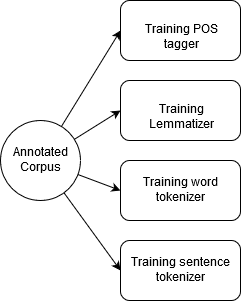
\includegraphics[scale=0.5]{cltk_pipelines-cltk_pipelines_training.png}    
\end{center}

\end{frame}

\begin{frame}{CLTK pipelines}
\begin{center}
    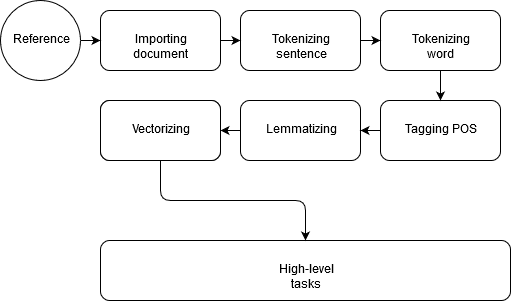
\includegraphics[scale=0.5]{cltk_pipelines-cltk_pipelines_executing.png}
    \end{center}
\end{frame}

% Generated with https://www.draw.io/


%\begin{frame}
%\begin{lstlisting}

%\end{lstlisting}


%\end{frame}


\subsection{Contribution}

\begin{frame}
\frametitle{Contribution}
\begin{itemize}
    \item Collaborative effort / open to a virtually infinite talent pool
    \item Avoid “re-inventing the wheel”
    \item Closer to the needs of the community
    \item Constant patches 
    \begin{itemize}
    \item Bugs are quickly resolved 
    \item New features are constantly developed
    
    \end{itemize}
    \item Transparency of development
    \item Generally results in safer software
    \item Easily customizable
\end{itemize}
\end{frame}

\begin{frame}
\frametitle{Why contribute?}
\begin{itemize}
    \item Best reason: ensure scientific reproducibility of your research
    \item Expand your skill set
    \item Give back to the community
    \item Open Source culture
    \item It’s Fun!
\end{itemize}
\end{frame}




\begin{frame}
\frametitle{How to contribute}
\begin{itemize}
    \item You can check out the \textbf{CLTK tutorials}\footnote{\href{https://github.com/cltk/tutorials}{https://github.com/cltk/tutorials}} and \textbf{docs}\footnote{\href{http://docs.cltk.org}{http://docs.cltk.org}}
    \item Take a look at the \textbf{open issues}\footnote{\href{https://github.com/cltk/cltk/issues}{https://github.com/cltk/cltk/issues}} or simply make \textbf{your own contribution}\footnote{\href{https://github.com/cltk/cltk/pulls}{https://github.com/cltk/cltk/pulls}}.
    \item Don’t hesitate to ask for help in the \textbf{IRC channel}\footnote{\href{https://gitter.im/cltk/cltk}{https://gitter.im/cltk/cltk}}!
\end{itemize}
\end{frame}

\begin{frame}
\frametitle{Contribute with GSOC}
%See the 32nd slide
\begin{itemize}
    \item Open for all university students
    \item You can work on an open source project for the summer
    \item CLTK participated for 3 years (2016, 2017, 2018)
\end{itemize}
\end{frame}

\begin{frame}
\frametitle{Previous GSOC Projects}
\begin{itemize}
    \item Additional support Akkadian, Germanic languages, Old and Middle French
    \item Greek/Latin Backoff lemmatizers.
    \item Support of more synonyms, translations and word embeddings for Greek and Latin
    \item Annotation support for the CLTK Archive
\end{itemize}
\end{frame}


\begin{frame}
\frametitle{CLTK Stats}
\begin{itemize}
\item Hosted by Github \href{https://github.com/cltk/cltk}{https://github.com/cltk/cltk}
\item 2723 commits
\item 83 contributors
\item 73 watchers, 560 stars, 283 forks
\item 45 releases, current version 0.1.112
\item Code coverage 89%
\end{itemize}


\end{frame}



\begin{frame}
\frametitle{Summary}
\begin{itemize}
    \item Digital tools can be used to aid academics and speed up mundane and well-defined processes
    \item Classical languages have their own unique set of challenges compared to modern languages
    \item CLTK offers an easy to use and well-documented API for Classical Natural Language Processing
\end{itemize}
\end{frame}


\begin{frame}
\begin{center}
    Thank you for your attention!\footnote{{You can now get stickers! \footnotesize}}
\end{center}




\end{frame}


\begin{frame}

\frametitle{Bibliography}
\begin{itemize}
    \item \label{paper:krauwer2003} Krauwer, S. 2003. “The Basic Language Resource Kit (BLARK) as the First Milestone for the Language Resources Roadmap.” Proceedings of the 2003 International Workshop on Speech and Computer (SPECOM 2003) : 8-15; cf. also Passarotti in SALTMIL 2010: 29.
    \item \label{paper:burns2019} Building a Text Analysis Pipeline for Classical Languages, https://www.degruyter.com/view/books/9783110599572/9783110599572-010/9783110599572-010.xml
\end{itemize}{}


\end{frame}


\begin{frame}
\frametitle{Contact us}

\begin{itemize}
\item Eleftheria Chatziargyriou, email address: \href{mailto:ele.hatzy@gmail.com}{ele.hatzy@gmail.com}, Github: \href{https://github.com/Sedictious}{Sedictious}

\item Clément Besnier, email address: \href{mailto:clemsciences@aol.com}{clemsciences@aol.com}, personal website: \href{https://www.clementbesnier.fr}{clementbesnier.fr}, Twitter: \href{https://twitter.com/clemsciences}{clemsciences}, Github: \href{https://github.com/clemsciences}{clemsciences}
\end{itemize}

\end{frame}


\begin{frame}
\nocite{*}
\bibliographystyle{amsalpha}
\bibliography{cltk.bib}
\end{frame}


% \begin{frame}
% \frametitle{Open source}
% \href{http://github.com}{github.com}
% Screenshot of the github code page.
% %like page 6

% \end{frame}

% \begin{frame}
% \frametitle{The docs}

% Screenshot of the docs

% \end{frame}


% \begin{frame}
% \frametitle{Project}


% Even if no lab is supporting it.

% Similar projects exist for living languages: SpaCy, NLTK, StanfordNLP, etc. Add links here 
% \end{frame}
% \section{CLTK as a tool for digital classics}

% \begin{frame}
% \frametitle{Gathers corpora from different sources}
% \begin{itemize}
%     \item annotated corpora
%     \item raw corpora
% \end{itemize}
% Some standardization
% \begin{itemize}
%     \item common encoding: UTF-8
%     \item 
% \end{itemize}


% CLTK comes after OCR\footnote{Optical Character Recognition} task.
% \end{frame}

% \begin{frame}
% \frametitle{Processes texts}
% \begin{itemize}
%     \item sentence segmentation
%     \item tokenization
%     \item POS tagging
%     \item lemmatization
    
% \end{itemize}
% \end{frame}

% \begin{frame}
% \frametitle{Ensuring quality}

% \begin{itemize}
%     \item reproducibility
%     \item collaborations
%     \item availability for all
    
% \end{itemize}

% \end{frame}

% \section{Example}
% \begin{frame}
% \frametitle{}


% \end{frame}

% \begin{frame}
% \frametitle{}


% \end{frame}


% \begin{frame}
% \frametitle{}


% \end{frame}


% \begin{frame}
% \frametitle{}


% \end{frame}


% \begin{frame}
% \frametitle{}


% \end{frame}


% \begin{frame}
% \frametitle{}


% \end{frame}




 
\end{document}